% Editable source for result.pdf, written by make_figures.py from run_github_39214027289/panel/result.json
\documentclass[tikz,border=6pt]{standalone}
\usepackage[T1]{fontenc}
\begin{document}
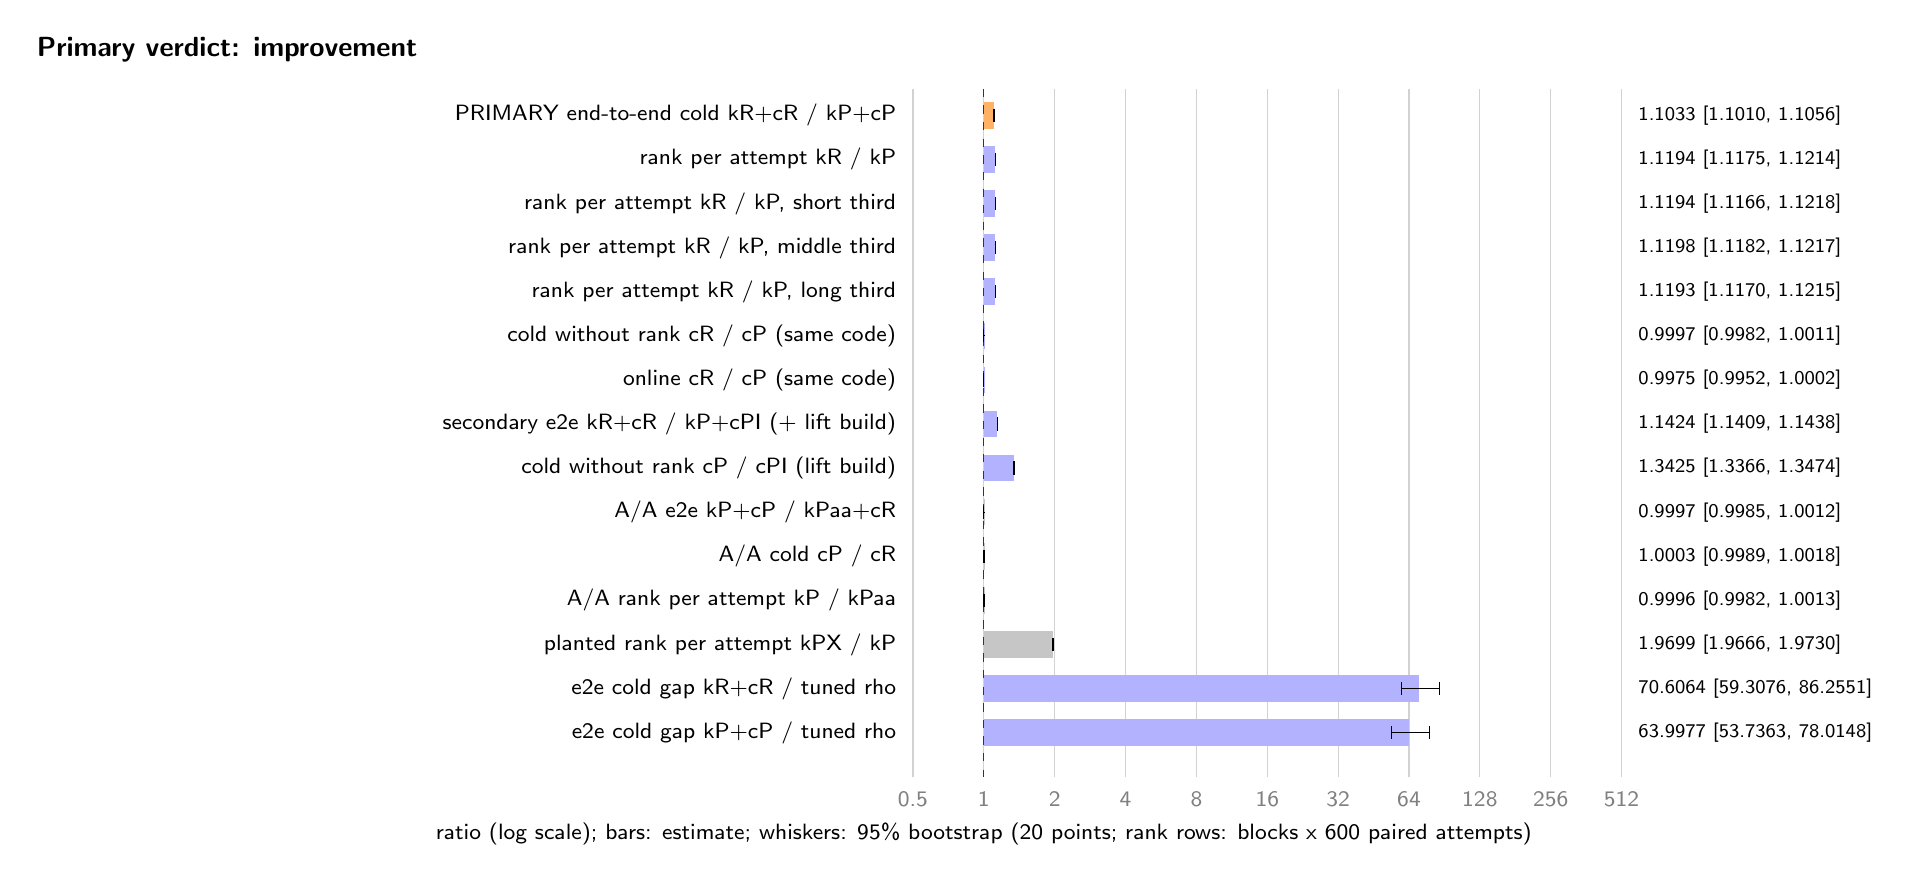
\begin{tikzpicture}[font=\sffamily\footnotesize,x=9mm,y=-5.6mm]
\draw[gray!35] (-1.0000,-0.6) -- (-1.0000,15); \node[gray] at (-1.0000,15.5) {0.5};
\draw[gray!35] (0.0000,-0.6) -- (0.0000,15); \node[gray] at (0.0000,15.5) {1};
\draw[gray!35] (1.0000,-0.6) -- (1.0000,15); \node[gray] at (1.0000,15.5) {2};
\draw[gray!35] (2.0000,-0.6) -- (2.0000,15); \node[gray] at (2.0000,15.5) {4};
\draw[gray!35] (3.0000,-0.6) -- (3.0000,15); \node[gray] at (3.0000,15.5) {8};
\draw[gray!35] (4.0000,-0.6) -- (4.0000,15); \node[gray] at (4.0000,15.5) {16};
\draw[gray!35] (5.0000,-0.6) -- (5.0000,15); \node[gray] at (5.0000,15.5) {32};
\draw[gray!35] (6.0000,-0.6) -- (6.0000,15); \node[gray] at (6.0000,15.5) {64};
\draw[gray!35] (7.0000,-0.6) -- (7.0000,15); \node[gray] at (7.0000,15.5) {128};
\draw[gray!35] (8.0000,-0.6) -- (8.0000,15); \node[gray] at (8.0000,15.5) {256};
\draw[gray!35] (9.0000,-0.6) -- (9.0000,15); \node[gray] at (9.0000,15.5) {512};
\draw[red!70!black,dashed] (0,-0.6) -- (0,15);
\node at (0,16.3) {ratio (log scale); bars: estimate; whiskers: 95\% bootstrap (20 points; rank rows: blocks x 600 paired attempts)};
\node[anchor=west,font=\sffamily\bfseries] at (-13.5,-1.5) {Primary verdict: improvement};
\node[anchor=east] at (-1.1000,0) {PRIMARY end-to-end cold kR+cR / kP+cP};
\fill[orange!60] (0,-0.300000) rectangle (0.1418,0.300000);
\draw (0.1388,0) -- (0.1448,0); \draw (0.1388,-0.150000) -- (0.1388,0.150000); \draw (0.1448,-0.150000) -- (0.1448,0.150000);
\node[anchor=west,font=\sffamily\scriptsize] at (9.1000,0) {1.1033 [1.1010, 1.1056]};
\node[anchor=east] at (-1.1000,1) {rank per attempt kR / kP};
\fill[blue!30] (0,0.700000) rectangle (0.1628,1.300000);
\draw (0.1603,1) -- (0.1653,1); \draw (0.1603,0.850000) -- (0.1603,1.150000); \draw (0.1653,0.850000) -- (0.1653,1.150000);
\node[anchor=west,font=\sffamily\scriptsize] at (9.1000,1) {1.1194 [1.1175, 1.1214]};
\node[anchor=east] at (-1.1000,2) {rank per attempt kR / kP, short third};
\fill[blue!30] (0,1.700000) rectangle (0.1628,2.300000);
\draw (0.1591,2) -- (0.1659,2); \draw (0.1591,1.850000) -- (0.1591,2.150000); \draw (0.1659,1.850000) -- (0.1659,2.150000);
\node[anchor=west,font=\sffamily\scriptsize] at (9.1000,2) {1.1194 [1.1166, 1.1218]};
\node[anchor=east] at (-1.1000,3) {rank per attempt kR / kP, middle third};
\fill[blue!30] (0,2.700000) rectangle (0.1632,3.300000);
\draw (0.1612,3) -- (0.1657,3); \draw (0.1612,2.850000) -- (0.1612,3.150000); \draw (0.1657,2.850000) -- (0.1657,3.150000);
\node[anchor=west,font=\sffamily\scriptsize] at (9.1000,3) {1.1198 [1.1182, 1.1217]};
\node[anchor=east] at (-1.1000,4) {rank per attempt kR / kP, long third};
\fill[blue!30] (0,3.700000) rectangle (0.1626,4.300000);
\draw (0.1596,4) -- (0.1654,4); \draw (0.1596,3.850000) -- (0.1596,4.150000); \draw (0.1654,3.850000) -- (0.1654,4.150000);
\node[anchor=west,font=\sffamily\scriptsize] at (9.1000,4) {1.1193 [1.1170, 1.1215]};
\node[anchor=east] at (-1.1000,5) {cold without rank cR / cP (same code)};
\fill[blue!30] (0,4.700000) rectangle (-0.0004,5.300000);
\draw (-0.0025,5) -- (0.0016,5); \draw (-0.0025,4.850000) -- (-0.0025,5.150000); \draw (0.0016,4.850000) -- (0.0016,5.150000);
\node[anchor=west,font=\sffamily\scriptsize] at (9.1000,5) {0.9997 [0.9982, 1.0011]};
\node[anchor=east] at (-1.1000,6) {online cR / cP (same code)};
\fill[blue!30] (0,5.700000) rectangle (-0.0036,6.300000);
\draw (-0.0069,6) -- (0.0002,6); \draw (-0.0069,5.850000) -- (-0.0069,6.150000); \draw (0.0002,5.850000) -- (0.0002,6.150000);
\node[anchor=west,font=\sffamily\scriptsize] at (9.1000,6) {0.9975 [0.9952, 1.0002]};
\node[anchor=east] at (-1.1000,7) {secondary e2e kR+cR / kP+cPI (+ lift build)};
\fill[blue!30] (0,6.700000) rectangle (0.1921,7.300000);
\draw (0.1901,7) -- (0.1938,7); \draw (0.1901,6.850000) -- (0.1901,7.150000); \draw (0.1938,6.850000) -- (0.1938,7.150000);
\node[anchor=west,font=\sffamily\scriptsize] at (9.1000,7) {1.1424 [1.1409, 1.1438]};
\node[anchor=east] at (-1.1000,8) {cold without rank cP / cPI (lift build)};
\fill[blue!30] (0,7.700000) rectangle (0.4249,8.300000);
\draw (0.4185,8) -- (0.4302,8); \draw (0.4185,7.850000) -- (0.4185,8.150000); \draw (0.4302,7.850000) -- (0.4302,8.150000);
\node[anchor=west,font=\sffamily\scriptsize] at (9.1000,8) {1.3425 [1.3366, 1.3474]};
\node[anchor=east] at (-1.1000,9) {A/A e2e kP+cP / kPaa+cR};
\fill[gray!45] (0,8.700000) rectangle (-0.0005,9.300000);
\draw (-0.0022,9) -- (0.0018,9); \draw (-0.0022,8.850000) -- (-0.0022,9.150000); \draw (0.0018,8.850000) -- (0.0018,9.150000);
\node[anchor=west,font=\sffamily\scriptsize] at (9.1000,9) {0.9997 [0.9985, 1.0012]};
\node[anchor=east] at (-1.1000,10) {A/A cold cP / cR};
\fill[gray!45] (0,9.700000) rectangle (0.0004,10.300000);
\draw (-0.0016,10) -- (0.0026,10); \draw (-0.0016,9.850000) -- (-0.0016,10.150000); \draw (0.0026,9.850000) -- (0.0026,10.150000);
\node[anchor=west,font=\sffamily\scriptsize] at (9.1000,10) {1.0003 [0.9989, 1.0018]};
\node[anchor=east] at (-1.1000,11) {A/A rank per attempt kP / kPaa};
\fill[gray!45] (0,10.700000) rectangle (-0.0006,11.300000);
\draw (-0.0026,11) -- (0.0019,11); \draw (-0.0026,10.850000) -- (-0.0026,11.150000); \draw (0.0019,10.850000) -- (0.0019,11.150000);
\node[anchor=west,font=\sffamily\scriptsize] at (9.1000,11) {0.9996 [0.9982, 1.0013]};
\node[anchor=east] at (-1.1000,12) {planted rank per attempt kPX / kP};
\fill[gray!45] (0,11.700000) rectangle (0.9781,12.300000);
\draw (0.9757,12) -- (0.9804,12); \draw (0.9757,11.850000) -- (0.9757,12.150000); \draw (0.9804,11.850000) -- (0.9804,12.150000);
\node[anchor=west,font=\sffamily\scriptsize] at (9.1000,12) {1.9699 [1.9666, 1.9730]};
\node[anchor=east] at (-1.1000,13) {e2e cold gap kR+cR / tuned rho};
\fill[blue!30] (0,12.700000) rectangle (6.1417,13.300000);
\draw (5.8901,13) -- (6.4305,13); \draw (5.8901,12.850000) -- (5.8901,13.150000); \draw (6.4305,12.850000) -- (6.4305,13.150000);
\node[anchor=west,font=\sffamily\scriptsize] at (9.1000,13) {70.6064 [59.3076, 86.2551]};
\node[anchor=east] at (-1.1000,14) {e2e cold gap kP+cP / tuned rho};
\fill[blue!30] (0,13.700000) rectangle (5.9999,14.300000);
\draw (5.7478,14) -- (6.2857,14); \draw (5.7478,13.850000) -- (5.7478,14.150000); \draw (6.2857,13.850000) -- (6.2857,14.150000);
\node[anchor=west,font=\sffamily\scriptsize] at (9.1000,14) {63.9977 [53.7363, 78.0148]};
\end{tikzpicture}
\end{document}
